% Asset ID: A21TrigonometryAndModellingTikZ-001
% Source: P2 Chapter 7 proof slide and teacher transcript
% Related section: Core Theory Part C
% Purpose: Geometric proof diagram for sin(A+B)

\documentclass[tikz,border=10pt]{standalone}
\usepackage{amsmath}
\usetikzlibrary{angles,quotes,calc,decorations.pathreplacing}
\begin{document}
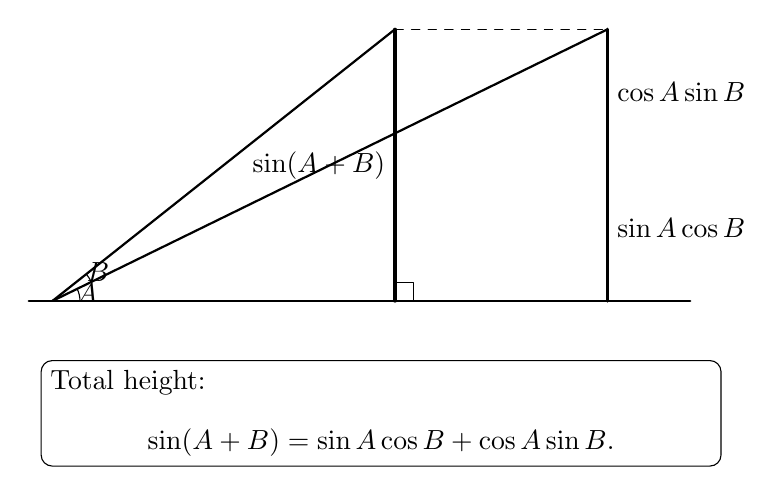
\begin{tikzpicture}[scale=3,line cap=round,line join=round]
\coordinate (O) at (0,0);
\coordinate (X) at (1.45,0);
\coordinate (Y) at (1.45,1.15);
\coordinate (P) at (2.35,1.15);
\coordinate (Q) at (2.35,0);
\coordinate (M) at (2.35,0.62);
\draw[thick] (-0.1,0)--(2.7,0);
\draw[thick] (O)--(Y);
\draw[thick] (O)--(P);
\draw[very thick] (X)--(Y);
\draw[dashed] (Y)--(P);
\draw[dashed] (P)--(Q);
\draw[very thick] (Q)--(M);
\draw[very thick] (M)--(P);
\draw (1.45,0) rectangle +(0.08,0.08);
\pic[draw,"$A$",angle radius=0.35cm,angle eccentricity=1.3] {angle=X--O--P};
\pic[draw,"$B$",angle radius=0.55cm,angle eccentricity=1.25] {angle=P--O--Y};
\node[left] at ($(X)!0.5!(Y)$) {$\sin(A+B)$};
\node[right] at ($(Q)!0.5!(M)$) {$\sin A\cos B$};
\node[right] at ($(M)!0.5!(P)$) {$\cos A\sin B$};
\node[draw,rounded corners,align=left,text width=8.4cm,anchor=north west] at (-0.05,-0.25)
{Total height:
\[
\sin(A+B)=\sin A\cos B+\cos A\sin B.
\]};
\end{tikzpicture}
\end{document}
